%---- Sample WMSU BSMATH BEAMER template ------
%---- Begin editing after PREAMBLE END at line 77------
%---- Created by: Christle Jude L. Maquilan - April 2022 --
%---- @jmaq03.jm@gmail.com -----

\documentclass[xcolor=dvipsnames,envcountsect]{beamer}

%-------- theme --------
\usetheme{Madrid}

%-------- color --------
\definecolor{peagreen}{RGB}{180,216,45}
\definecolor{darkpastelgreen}{rgb}{0.01, 0.75, 0.24}
\definecolor{pantone339}{RGB}{0, 178, 134}


\usecolortheme[named=pantone339]{structure}
%-------- set color of 'example block' to crimson theme --------
\setbeamercolor{block body example}{bg=white}
\setbeamercolor{block title example}{fg=white, bg=red!80!black}

%-------- font --------
\setbeamerfont{structure}{family=\rmfamily,series=\bfseries}
\usefonttheme[stillsansseriftext]{structurebold}
\setbeamerfont{section in head/foot}{size=\tiny}

%-------- misc structure --------
\useoutertheme[footline=authortitle,subsection=false]{miniframes}
\useinnertheme{rounded}
\addtobeamertemplate{block begin}{}{\justifying}
\newtheorem{remark}[theorem]{Remark}
\renewcommand{\indent}{\hspace*{2em}}
\setbeamertemplate{theorems}[numbered]
\setbeamertemplate{caption}[numbered]
\usepackage[justification=centering]{caption}
\renewcommand{\qedsymbol}{$\blacksquare$}

%-------- packages to be used -------
\usepackage{amsmath,amsfonts,amssymb,amscd,amsthm}
\usepackage{booktabs}
\usepackage{cclicenses}
\usepackage{graphicx,xcolor,comment}
\usepackage{mathrsfs} 
\usepackage{multirow}
\usepackage{array}
\usepackage{hyperref}
\usepackage{multicol}
\usepackage{ragged2e}
\usepackage{caption}
\usepackage[english]{babel}
\usepackage{rotating}
\usepackage{enumerate}
\usepackage{tikz}
\usepackage{bm}
\usepackage{csquotes}
\usepackage{gensymb,textcomp,mathcomp}
\usepackage{textcomp}

\graphicspath{{Figures}}

\newcommand{\flushdown}{\vskip0pt plus 1filll}

%-------- for bibliography -----------------
\usepackage{biblatex}
\setbeamertemplate{bibliography item}{\insertbiblabel}
\addbibresource{main2_references.bib}
\setbeamertemplate{frametitle continuation}{\frametitle{\color{white}List of References}}
% remove section headline
\setbeamertemplate{headline}{}

\newcommand{\backupbegin}{
   \newcounter{framenumberappendix}
   \setcounter{framenumberappendix}{\value{framenumber}}
}
\newcommand{\backupend}{
   \addtocounter{framenumberappendix}{-\value{framenumber}}
   \addtocounter{framenumber}{\value{framenumberappendix}} 
}
\newcommand{\licensecc}{\href{https://en.wikipedia.org/wiki/Creative\_Commons}{\cc}}
\newcommand{\licenseccA}{\href{https://creativecommons.org/licenses/by/4.0/deed.en}{\ccAttribution}}
\newcommand{\licenseccS}{\href{https://en.wikipedia.org/wiki/Share-alike}{\ccShareAlike}}

\newcommand\Tstrut{\rule{0pt}{2.6ex}}         % = `top' strut
\newcommand\Bstrut{\rule[-0.9ex]{0pt}{0pt}}   % = `bottom' strut
\newcommand{\adenine}{{\tt A}}
\newcommand{\cytosine}{{\tt C}}
\newcommand{\guanine}{{\tt G}}
\newcommand{\thymine}{{\tt T}}
\newcommand\kmer{{\it k}-mer}
\newcommand\kmers{{\it k}-mers}

\title[What is in my Sample?]{What is in my Sample? – Challenges and Approaches for Unveiling the Hidden Diversity in Plankton Samples}

\author [Hoffmann, Marie]{\textbf{Marie Hoffmann (MSc Computer Science)}}

\institute[Western Mindanao State University] {\emph{Advisers: }\textbf{Prof. Knut Reinert, Prof. Michael T. Monaghan}\\[1em]
	Department of Mathematics and Computer Science\\Free University Berlin\\[1em]

\includegraphics[scale=0.06]{./Figures/fu_logo5.png}}

\date[August 23, 2022]{\footnotesize Disputation - \textbf{August 23, 2022}}
%--------- DURATION 20 MIN ------------------

\begin{document}
	
\begin{frame}{\titlepage}\end{frame}
% \begin{frame}{\frametitle{Presentation Outline}\tableofcontents}\end{frame}


%--------- INTRODUCTION ----------------------
\section{Metabarcoding} % Motivation
\subsection{Motivation}
% \begin{frame}\frametitle{Motivation}
\begin{frame}{Motivation: Lake Monitoring Project}
\framesubtitle{Conducted at IGB Berlin}
\begin{figure}
    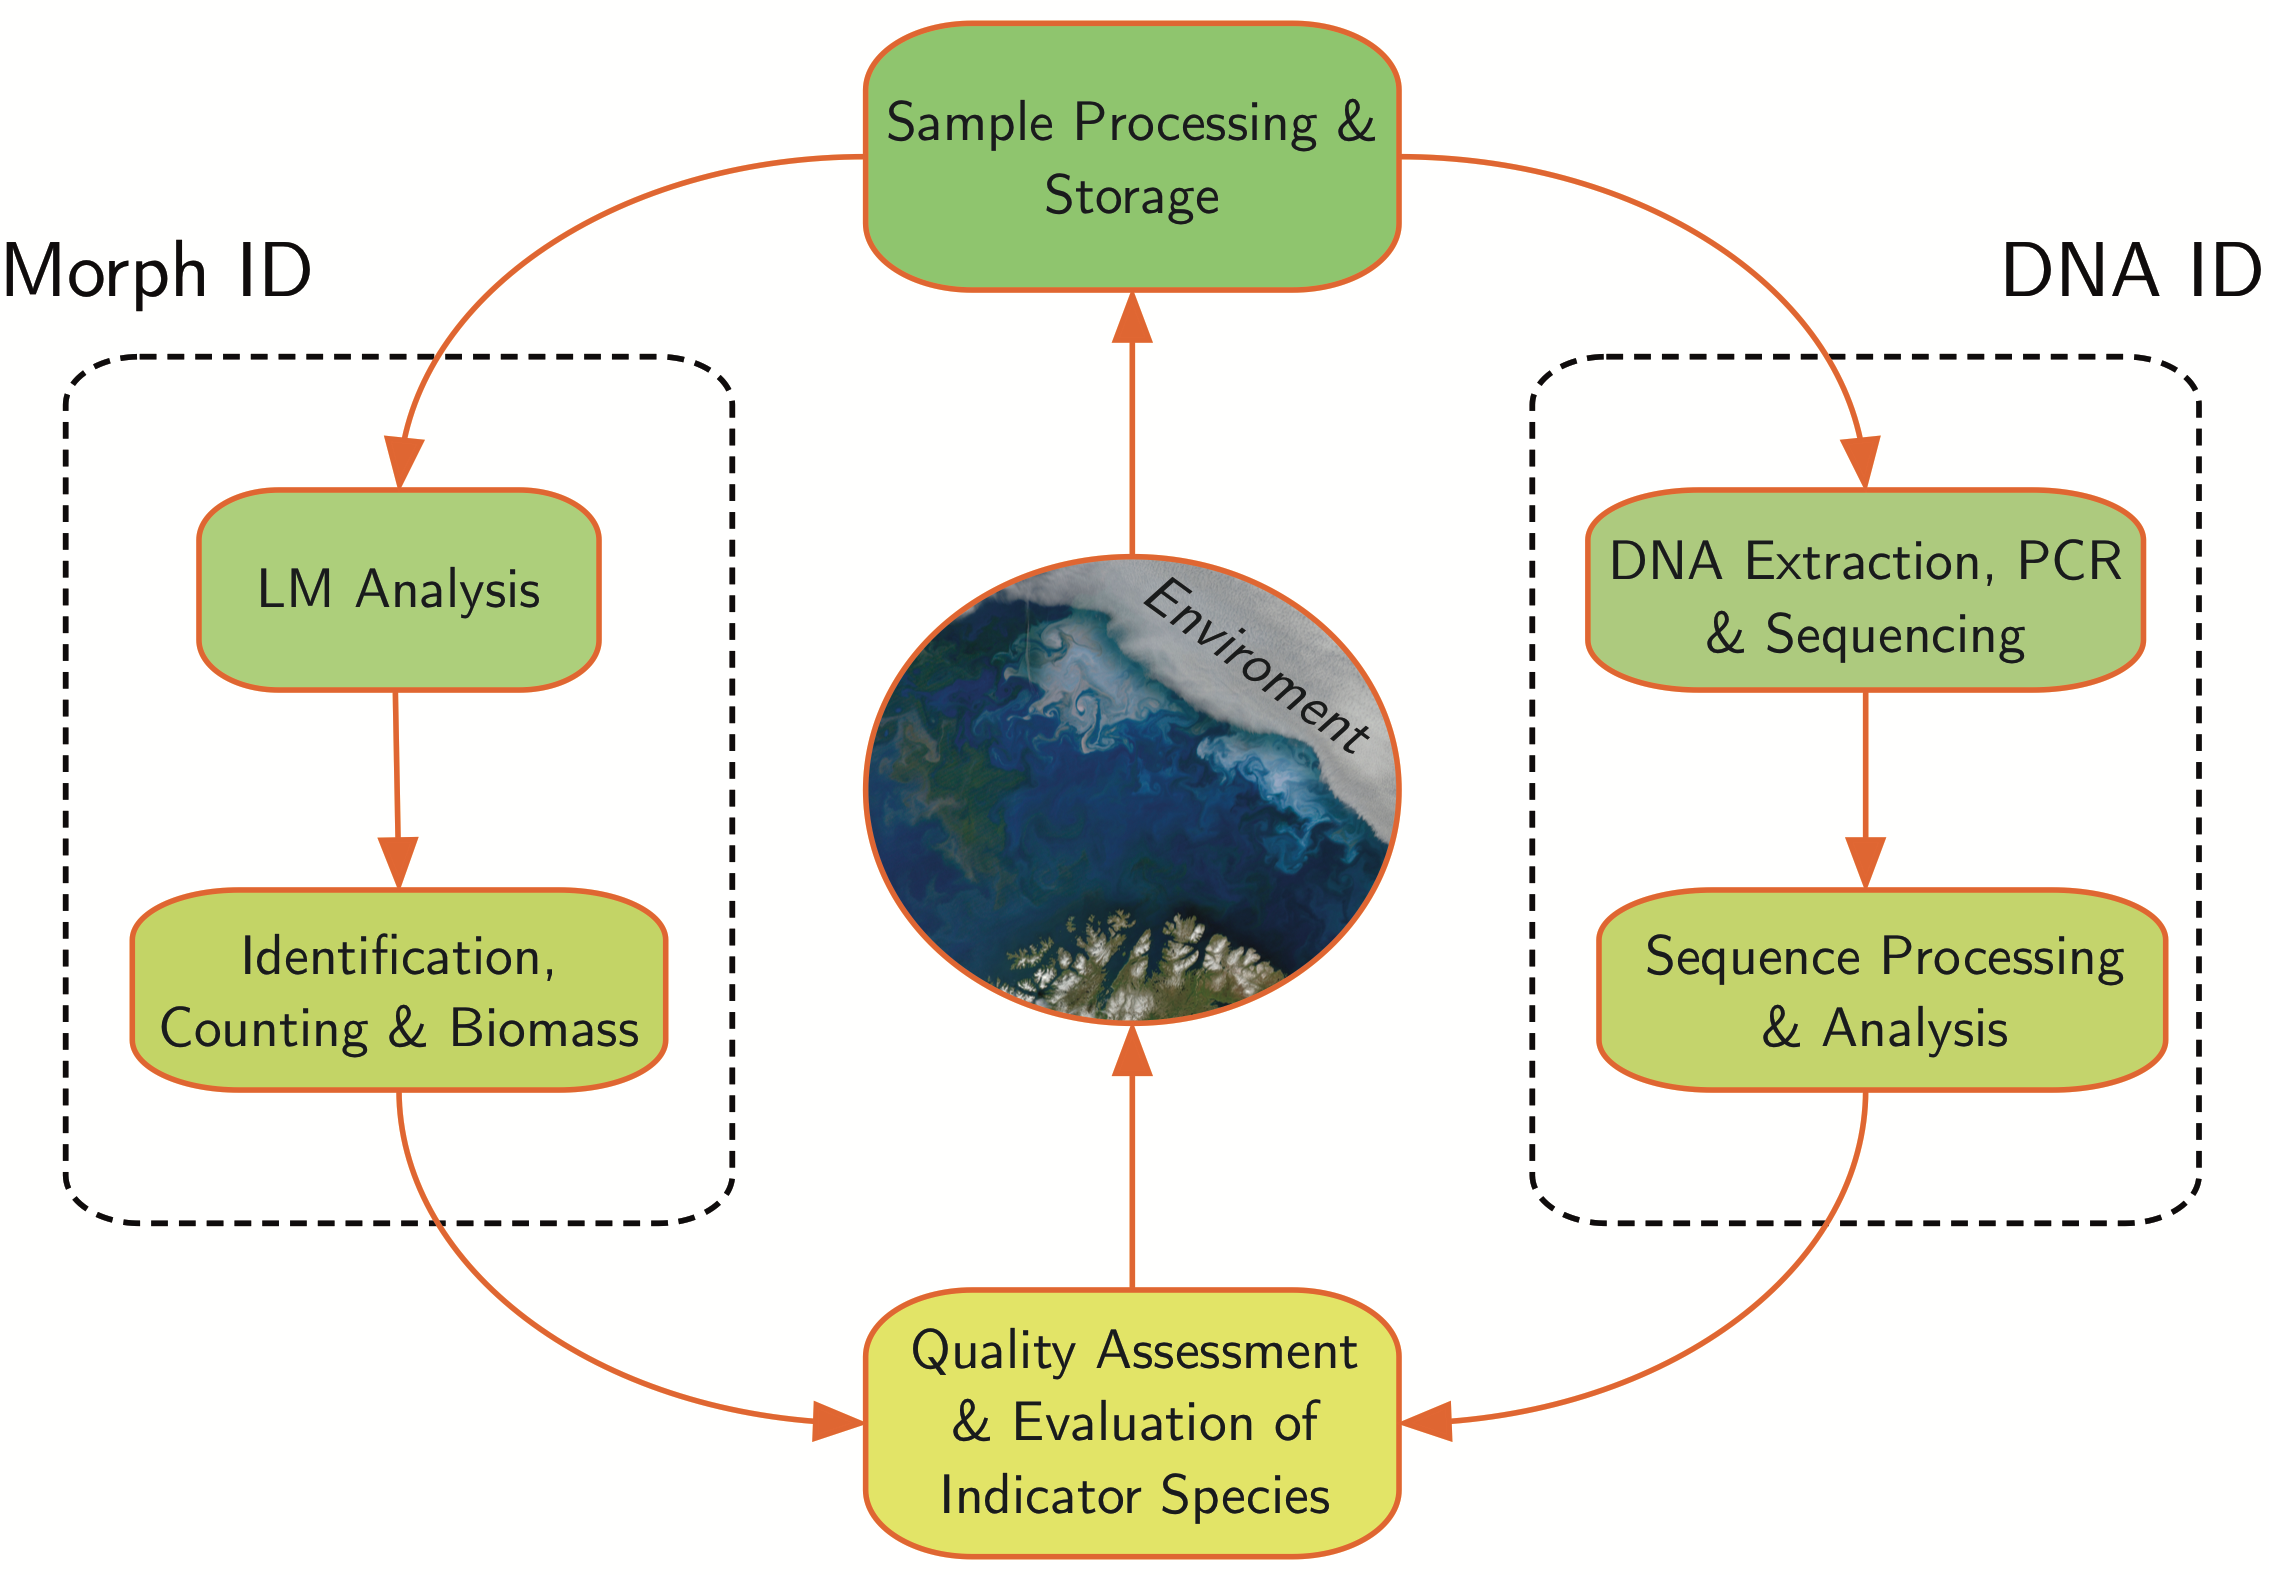
\includegraphics[scale=.6]{sample_processing}
    \caption{Complementing processing pipeline to study dynamics of freshwater samples.}
\end{figure}
\end{frame}

% longterm goal: optimize the combination of primers used in the protocol w.r.t. relevant species, but also broadness - sensitivity towards new trends, invasive, or poisonous species
% less identification tasks are necessary by human experts, but focus on description of unknown species, teratological forms, biomass estimation

\begin{frame}{Motivation: Lake Monitoring Project}
\framesubtitle{Challenge: Species Diversity}
\begin{figure}
    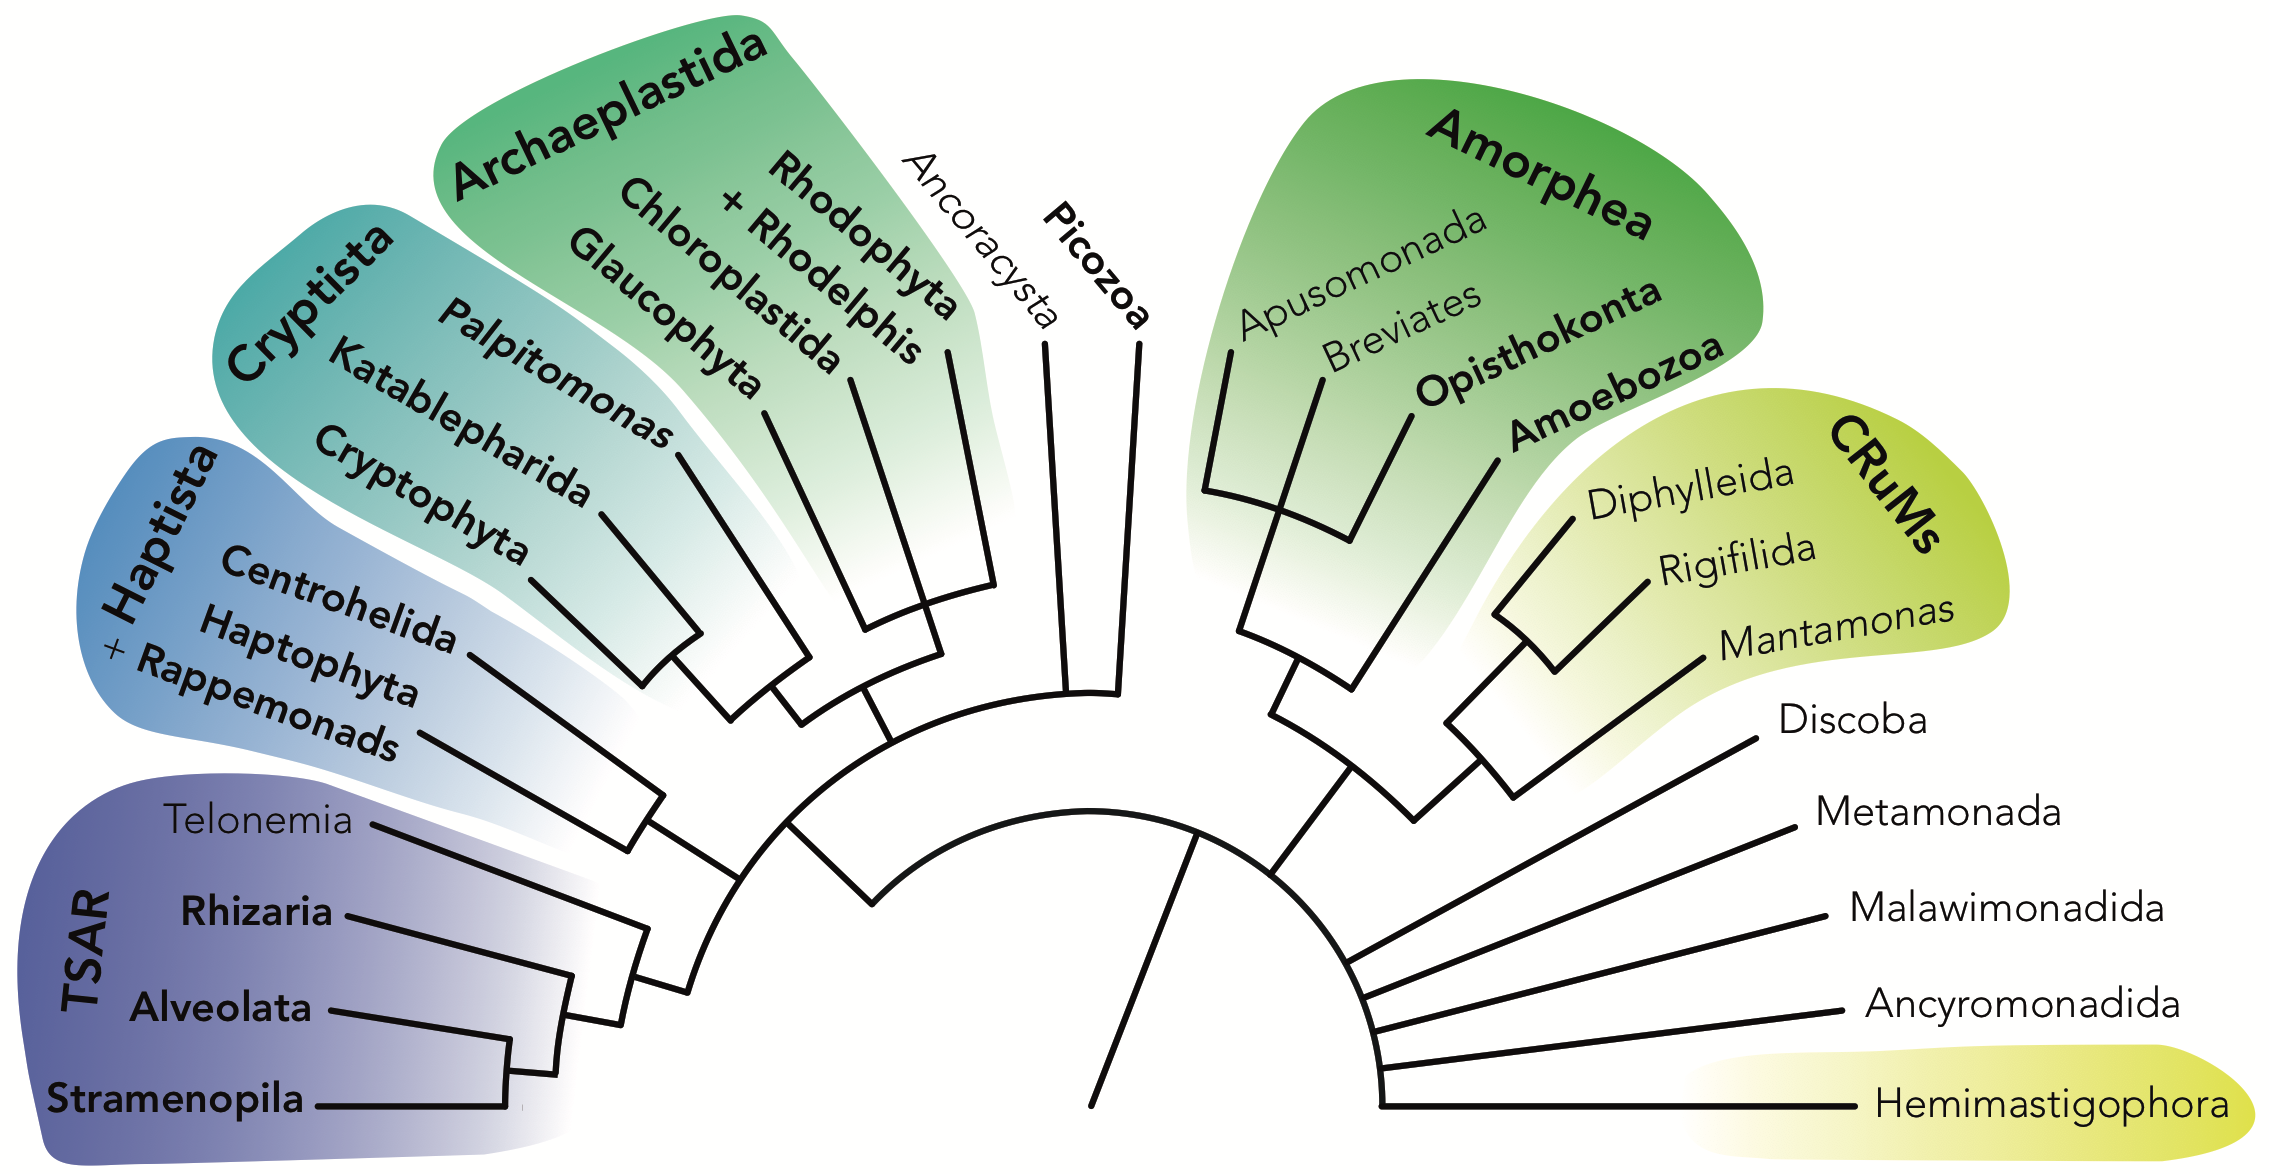
\includegraphics[scale=.6]{eTOL2}
    \caption{Dendrogram of the eukaryote tree of life proposed by \cite{Burki2020}.}
\end{figure}
\end{frame}

% Supergroups of the eurkaryote tree of life 
% based on phylogenetic differences
% there exists multiple taxonomic trees, relevant when resolving to higher taxa above species, Consolidation: No unique, generally accepted taxonomic
% Challenges in protocol enhancement
% capturing taxonomic {\it width} versus {\it depth} % Taxonomic heterogeneity 
% Optimization: Missing ground truth % => need to remain sensitive, unbiased
% Resolution: Databases are sparse, erroneous, uncurated % partial sequences, rarely complete genomes
%     \item  tree!  % if consulting multiple databases to maximize ID
%     % \item Few human experts available (to support complementation of unlabeled sequences)
%     \item  PCR: Same difficulties as single organisms DNA analysis: repeats, intra-species variation, ...
% \end{enumerate}
% \end{frame}

\begin{frame}\frametitle{Motivation: Lake Monitoring Project}
\framesubtitle{Study Design}
\begin{multicols}{2}
Pooled samples underwent both 
\begin{itemize}
    \item Morph ID 
    \item DNA ID with three markers
\end{itemize}\begin{table}\centering
\small
    \begin{tabular}{llc}
    \toprule
    \small Marker ID &\small Name &\small Ref. \\
    \hline\toprule
    \multirow{2}{*}{EUK15} &\footnotesize TAReuk454FWD1 &\multirow{2}{*}{\cite{Stoeck2010}} \\
    &\footnotesize TAReukREV3 & \\\hline\Tstrut
    \multirow{2}{*}{EUK14} &\footnotesize F-566a & \multirow{2}{*}{\cite{Hadziavdic2014}} \\
    &\footnotesize R-1200 & \\\hline\Tstrut
    \multirow{2}{*}{DIV4} &\footnotesize DIV4for & \multirow{2}{*}{\cite{Visco2015}} \\
    &\footnotesize DIV4rev3 & \\\bottomrule
\end{tabular}\caption{Primers for metabarcoding on freshwater plankton samples.}\label{Tab:primer2}
\end{table}
% \columnbreak
\begin{figure}\center
    \includegraphics[scale=.4]{MC_Sampler}\caption{Integrated water sampler. \copyright HYDRO-BIOS Apparatebau GmbH}
\end{figure}
\end{multicols}
\end{frame}
% all primers target V4 region of the 18S rRNA gene
% EUK15 target all groups of Eukaryota except Excavata and Microsporidia
% EUK14 target marine sediment communities
% DIV4 diatoms

\begin{frame}\frametitle{Motivation: Lake Monitoring Project}
\framesubtitle{Study Results: Number of Taxa}

\begin{table}[htpb]\centering
\begin{tabular}{lcccccc}\toprule
&& \multirow{2}{*}{Taxa/OTU} && Genus && Species\\
&& && Level ID && Level ID \\\toprule
Morph ID && 235 && 206 (88 \%)&& 146 (62 \%) \\
EUK15 ID && 325 && 277 (69 \%) && 128 (40 \%) \\
EUK14 ID && 506 && 268 (53 \%) && 166 (33 \%) \\
DIV4 ID && 543 && 344 (63 \%) && 231 (43 \%) \\\bottomrule
\end{tabular}
\caption{Number of taxa (Morph ID) and OTUs (molecular ID) found and identified to genus or species level. } \label{Tab:Tab_2} % Note that the counters are hierarchical, i.e. genera counts include species.
% at first glance this looks promising, 
% table does not tell us about the amount of overlap
\end{table}

\end{frame}

\begin{frame}\frametitle{Motivation: Lake Monitoring Project}
\frametitle{Key Findings Morph ID vs DNA ID}
\begin{columns}
\column{.7\textwidth}
Morph ID
\begin{itemize}
    \item number of $\text{species} \in \{\text{Morph ID} \} \backslash \{ \text{DNA ID}\} = 141$
    \item Unbiased towards abundant organisms % well-studied
    \item Allows biomass estimation
\end{itemize}
DNA ID
\begin{itemize}
    \item better presence/absence test of species % higher diversity, but no abundance information, even on fungi
    \item sensitive to spurious, invasive species, fungi
    \item Species remain undetected if 
    \begin{itemize}
        \item primers insufficiently match 
        \item similarity threshold low for OTU formation
        \item {\bf Phylum of rotifers undetected}
    \end{itemize}
\end{itemize}
% Undetected group: rotifera
\column{.3\textwidth}
\begin{figure}\centering
    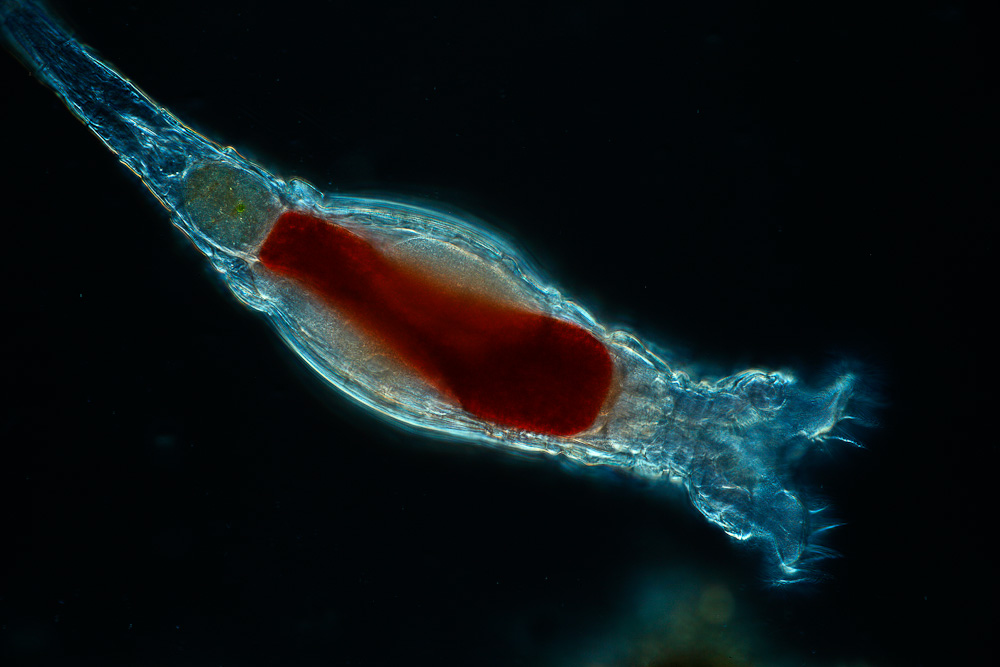
\includegraphics[scale=.4]{rotifer}\caption{Rotifer. \licensecc BY-SA 3.0 de from Wikipedia.}
\end{figure}
\end{columns}
\end{frame}


\begin{frame}{Motivation: Lake Monitoring Project}
\framesubtitle{Desiderium for Ongoing Protocol Enhancement}
\begin{enumerate}[I]
    \item Robust {\it de novo} primer discovery and {\it in silico} evaluation % understanding its efficiency
    \begin{itemize}
        \item Automated proto-primer search in uncurated databases % like NCBI’s nt dataset
        \item Robust to sequencing errors
        \item Preference for high-frequent proto-primers % as a proxy for coverage of a specific clade
    \end{itemize}
\end{enumerate}
\begin{figure}
    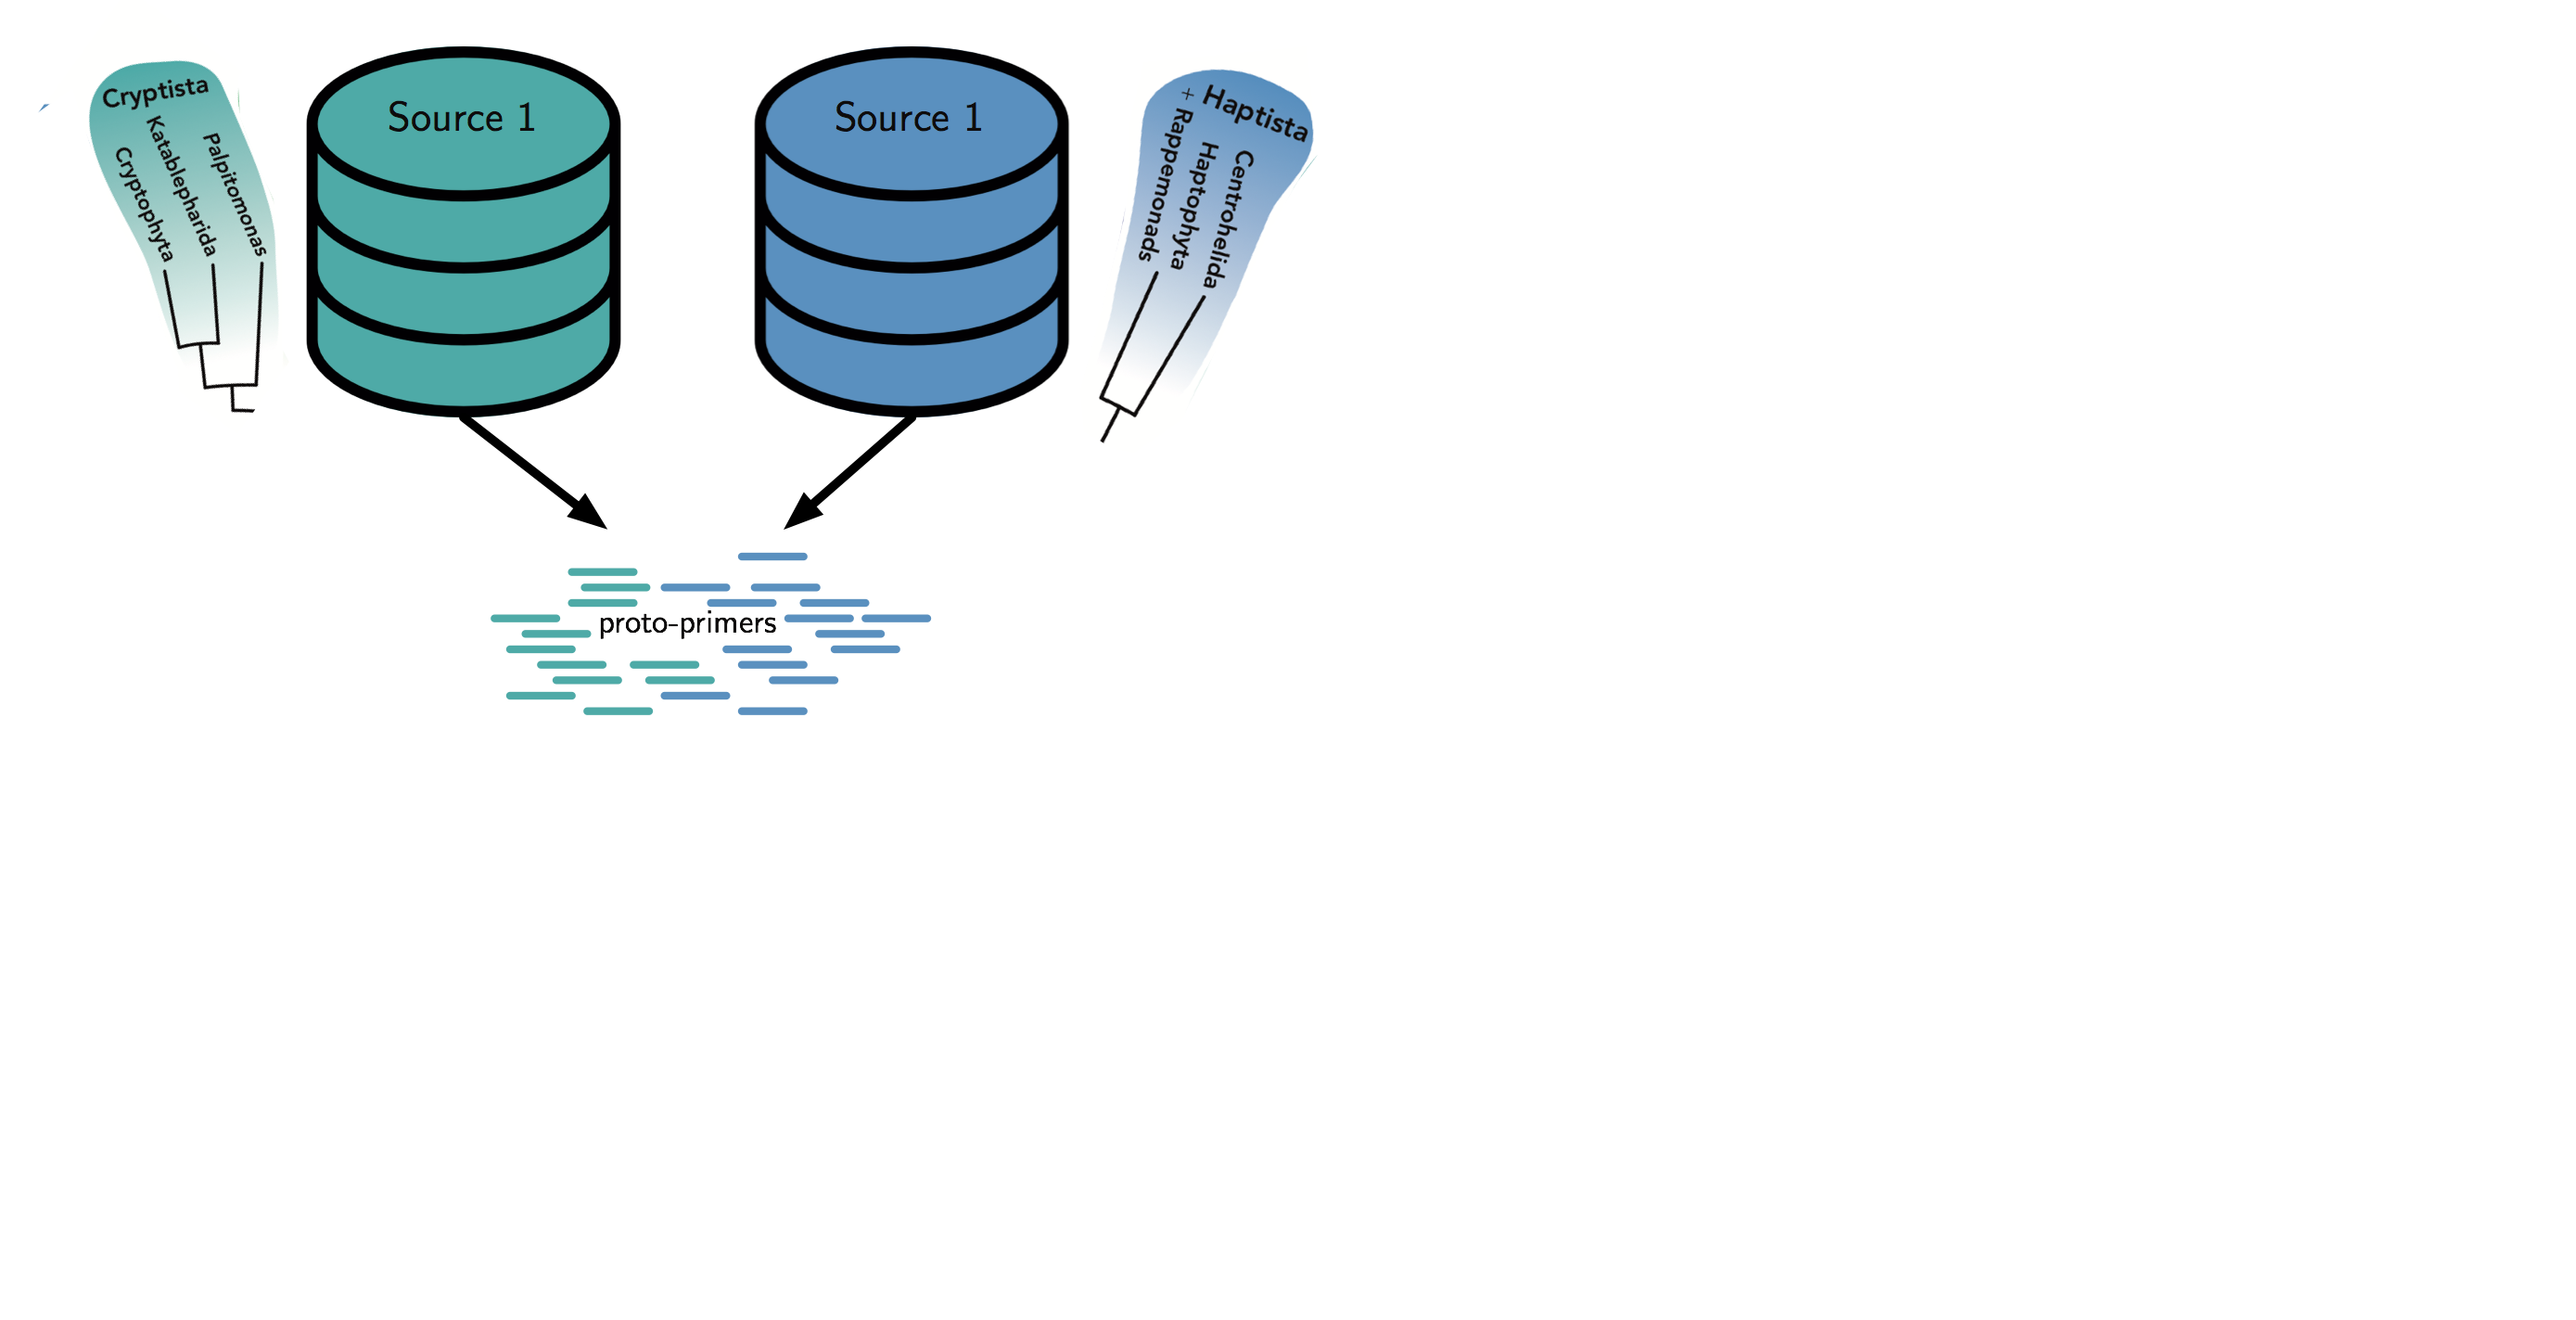
\includegraphics[scale=.4]{DB_protoprimers}
\end{figure}
\end{frame}

% cubic in n for T-Coffee O(n2l2) + O(n3l)

\begin{frame}{Robust Primer Discovery}
\framesubtitle{How to make it computational feasible?}
% \framesubtitle{Primer Search Tool: PriSeT \cite{PriSeTGitHub}}
\begin{block}
	\scshape
Idea: Avoid MSA, but search for frequent k-mers (=proto-primers)
\end{block}
%  T-Coffee for MSA computations consumes O(n2l2) + O(n3l)
% 15k Chlorophyta -> n^3 = 3.4 x 10^12 -> Dikarya: 209,449
%Challenge: amount of primer candidates derivable from database
% MSA are sensitive to sequence errors
    \begin{enumerate}
        \item Build FM-index \cite{Ferragina2005} on $T = R_1 \circ  R_2 \circ \cdots \circ R_m$  % combines the Burrows-Wheeler compression algorithm (BW, see Burrows and Wheeler, 1994) and suffix arrays (SAs) to obtain a compressible
        \begin{itemize}
            \item FM-index provides
            \begin{eqnarray*}
            \operatorname{locate} (T, \operatorname{kmer}) &:=& A[l:r]\\
            \operatorname{frequency} (T, k) &:=& [r_i - l_i + 1]_{i\in [1:|T|]}
            \end{eqnarray*}
            with $l_i$, $r_i$ denoting the ranges for k-mer $T[i:i+k-1]$
        \end{itemize}
        \item Lookup k-mers with minimal frequency threshold % 10^6 - 10^7 k-mers
    \end{enumerate}
    % TODO: illustration
% \vskip0pt plus 1filll
\flushdown
\rule{\textwidth}{.8pt} 
{\footnotesize
\begin{description}
    \item[$R_i$] reference sequence
    \item[$k$] target length for proto-primer
    \item[kmer] = proto-primer
    \item[$A$] suffix array derived from text $T$ 
\end{description}
}
\end{frame}

\begin{frame}{Robust Primer Discovery}
\framesubtitle{How to make it computational feasible?}
% \framesubtitle{Primer Search Tool: PriSeT \cite{PriSeTGitHub}}
Primer fitness test
\begin{enumerate}
    \item Two-bit encoding scheme $\texttt{A}\mapsto 00$, $\texttt{C}\mapsto 01$,  $\texttt{G}\mapsto 10$, $\texttt{T}\mapsto 11$ %(Fig. \ref{TKMerID})
    \item<2> Bit-parallelism %(Fig. \ref{bitparallel_CG})
\end{enumerate}
\only<1>{
    \begin{figure}
        \includegraphics[scale=.3]{TKMerID}
        \caption{K-mer compression scheme.}\label{TKMerID}
    \end{figure}
}
\only<2>{
    \setcounter{figure}{3}
    \begin{figure}
        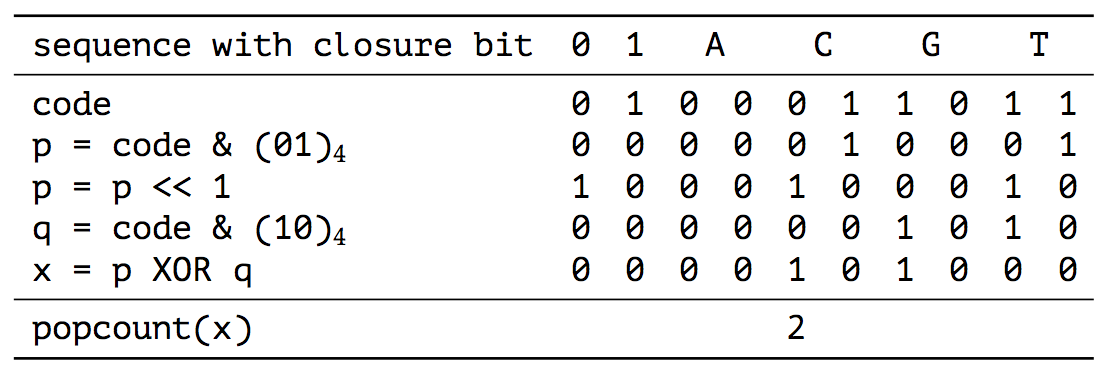
\includegraphics[scale=.5]{bitparallel_CG}
        \caption{Bit-parallelized counting of CG.}\label{bitparallel_CG}
    \end{figure}
}
\flushdown
Presented techniques implemented in PriSeT \cite{PriSeTGitHub}.
\end{frame}

\begin{frame}{Robust Primer Discovery}
\framesubtitle{Evaluation on Plankton Dataset: Library}
\begin{figure}
    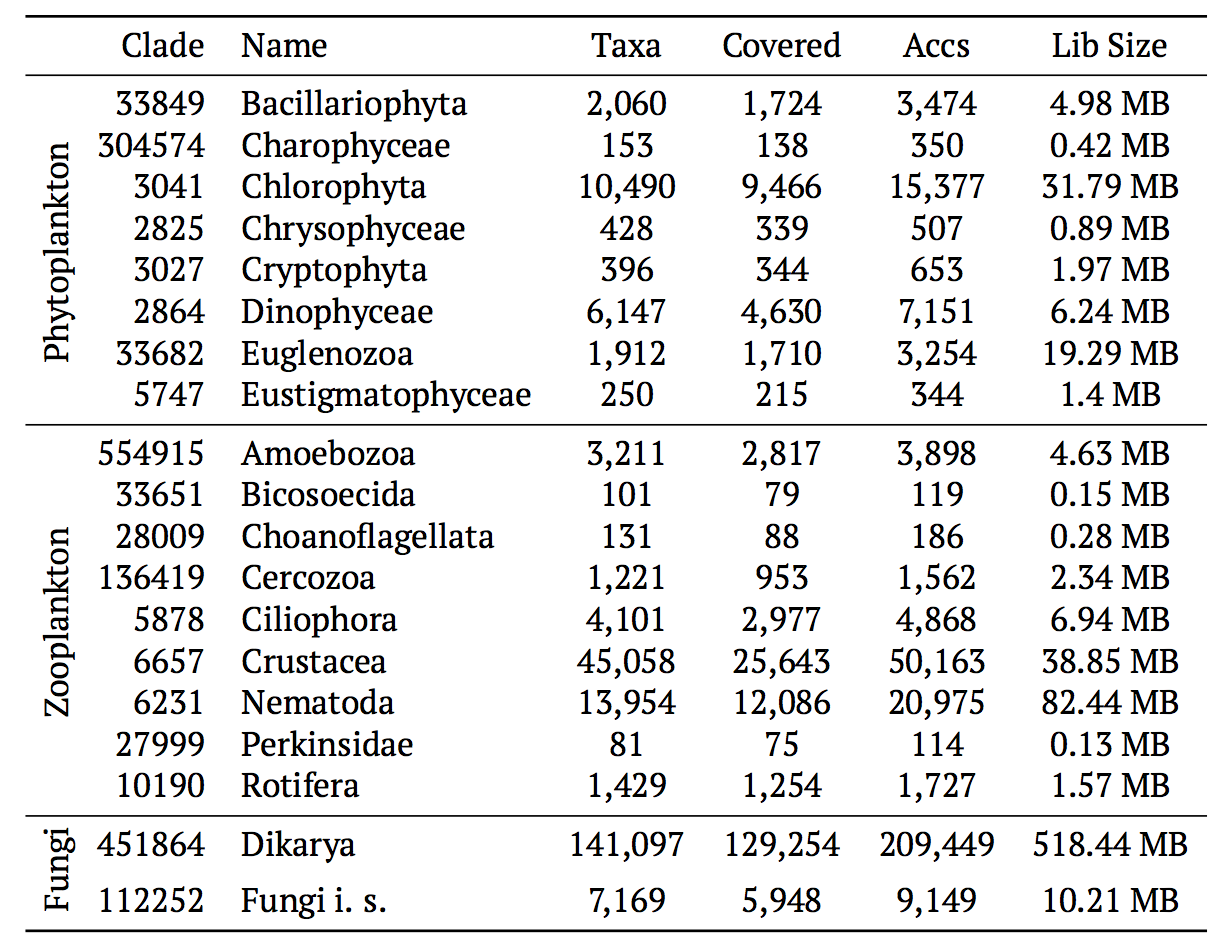
\includegraphics[scale=.38]{plankton_data}
    \caption{Reference sequences sampled from plankton taxa as found in GenBank's nt dataset.}
\end{figure}
% \hfill
\end{frame}

% \begin{frame}{I Robust Primer Discovery}
\begin{frame}{Robust Primer Discovery}
\framesubtitle{Evaluation on Plankton Dataset: comparison of proto-primer}
\begin{figure}\centering
    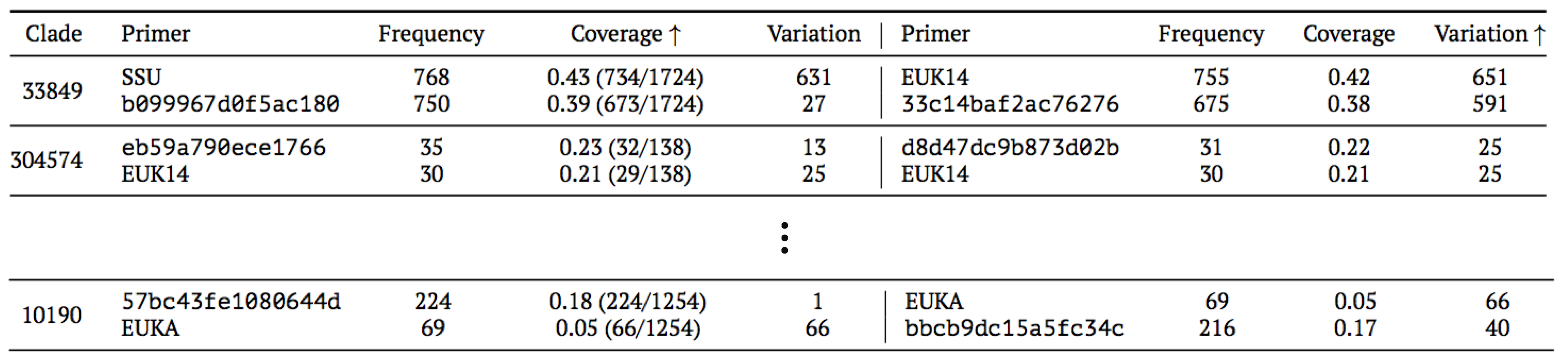
\includegraphics[scale=.47]{denovo_plankton}
    \caption{Excerpt from table of computed proto-primers (16-digits) compared to published primer pairs (SSU, EUK14, EUKA). Coverage: number of sequences covered. Variation: number of unique amplicon.}
\end{figure}
Results: at least one new primer pair identified by PriSeT
\begin{itemize}
    \item Ranking by coverage: for 11 / 19 clades %, PriSeT identifies at least one new primer pair with a higher coverage rate % than the published primers
% \hfill
    \item Ranking by amplicon variation: for 7 / 19 clades %, PriSeT found at least one more or equally performant primer pair
\end{itemize}
% given that the rSSU is already a well studied and exploited region, is not too bad
\end{frame}

% \begin{frame}{I Robust Primer Discovery}
\begin{frame}{Robust Primer Discovery}
\framesubtitle{Evaluation on Plankton Dataset: Runtime of proto-primer generation}
\begin{figure}\centering
    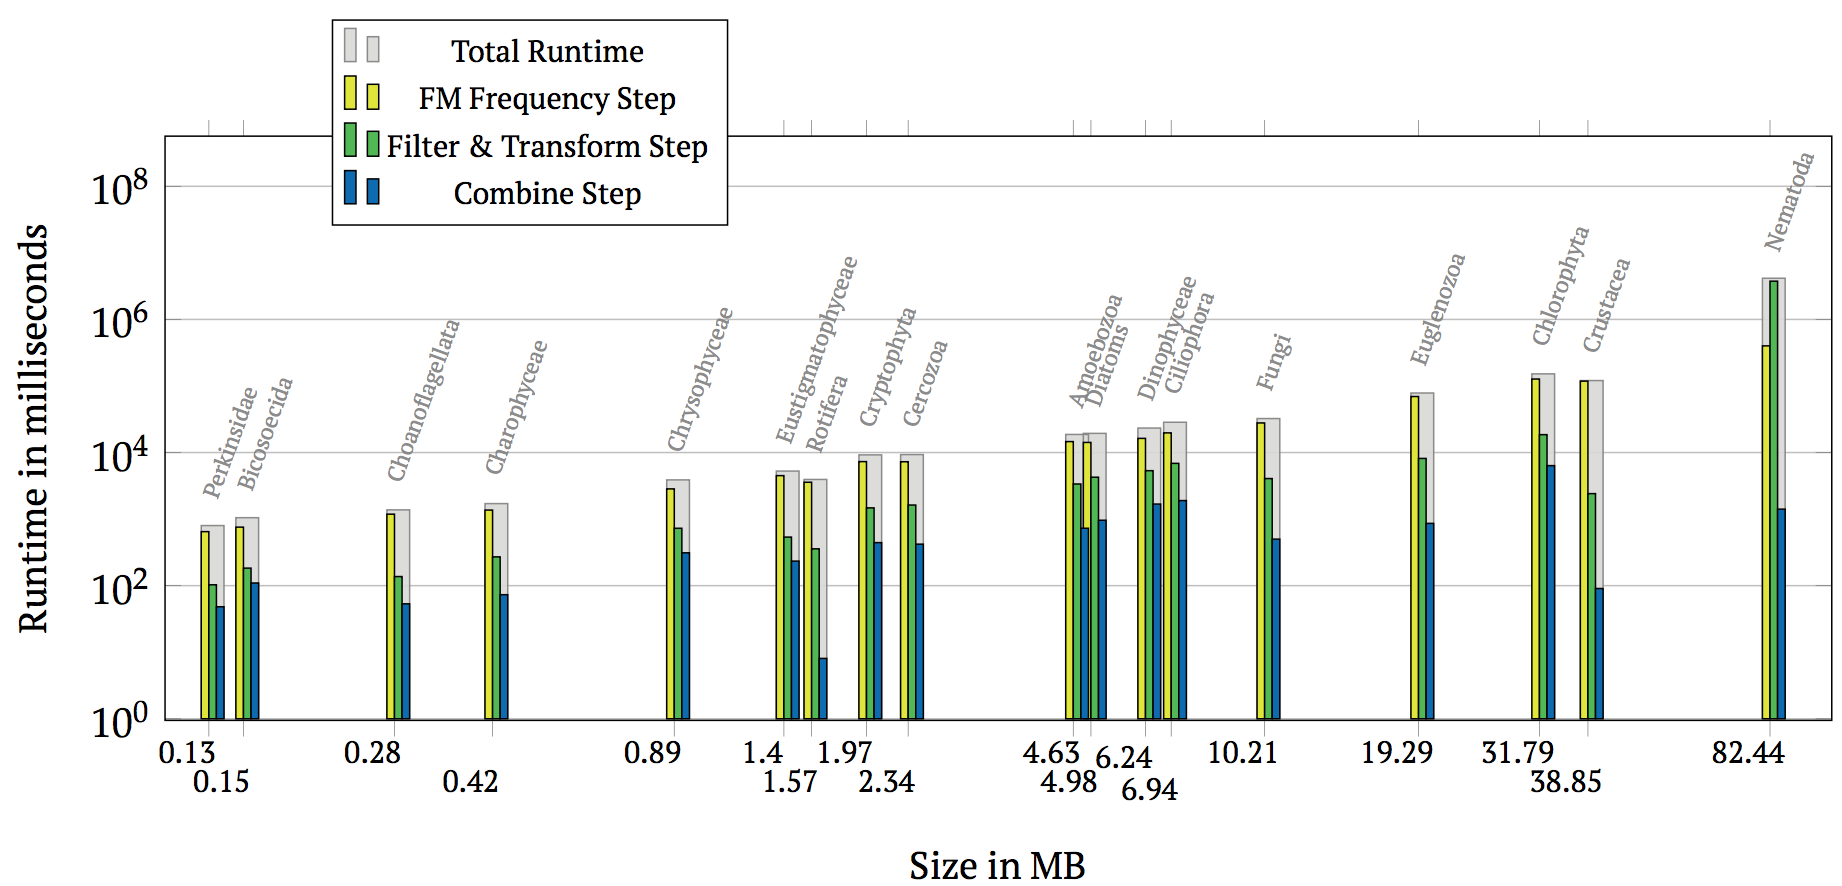
\includegraphics[scale=.36]{plankton_runtime}
    \caption{Runtimes for plankton clades vary from about 1 sec (Perkinsidae) to 15 min (Nematoda).}
\end{figure}
\end{frame}

% \begin{frame}{I Robust Primer Discovery}
\begin{frame}{Robust Primer Discovery}
\framesubtitle{Theoretical Runtime and Space Consumption}
\begin{table}[htpb]\centering
\begin{tabular}{@{}rcc@{}}\toprule
&       FM-Index & FM Frequency\\ \midrule
Runtime & $\mathcal{O}(N)$ & $O(N(\kappa_{\max} + occ))$ \\\Tstrut
Space   & $\mathcal{O}(\log |\Sigma| N) + o(\log|\Sigma|^2N)$ & $\mathcal{O}(N)$ \\
\toprule
 & Filter \& Transform & Combine \\ \midrule
Runtime & $\mathcal{O}(\kappa_{\max}N)$ & $\mathcal{O}(n\kappa_{\max}(\frac{N}{n} - \tau_{min})(\tau_{max} - \tau_{min}))$ \\
Space & $\mathcal{O}(N)$ & $\mathcal{O}(n(\frac{N}{n} - \tau_{min})(\tau_{max} - \tau_{min}))$ \\
\bottomrule
\end{tabular}
\caption{Runtime classes and space occupation module-wise with $N$ as the total library size, $|\Sigma|$ is four, because of the underlying alphabet being $\{ \adenine , \cytosine, \guanine, \thymine \}$, $n$ the number of references per library, $\kappa_{\max}$ the largest \kmer{} length, $\omega$ the window width, and $\tau_{\text{min/max}}$ the amplicon length limits, and $occ$ the expected number of \kmer{} occurrences.} \label{Tab:runtimes2}
\end{table}
\end{frame}

\begin{frame}{Robust Primer Discovery}
\framesubtitle{Evaluation on SARS-CoV-2}
PriSeT: 286 proto-primers in total, 114 with unique transcripts
\begin{figure}\centering
    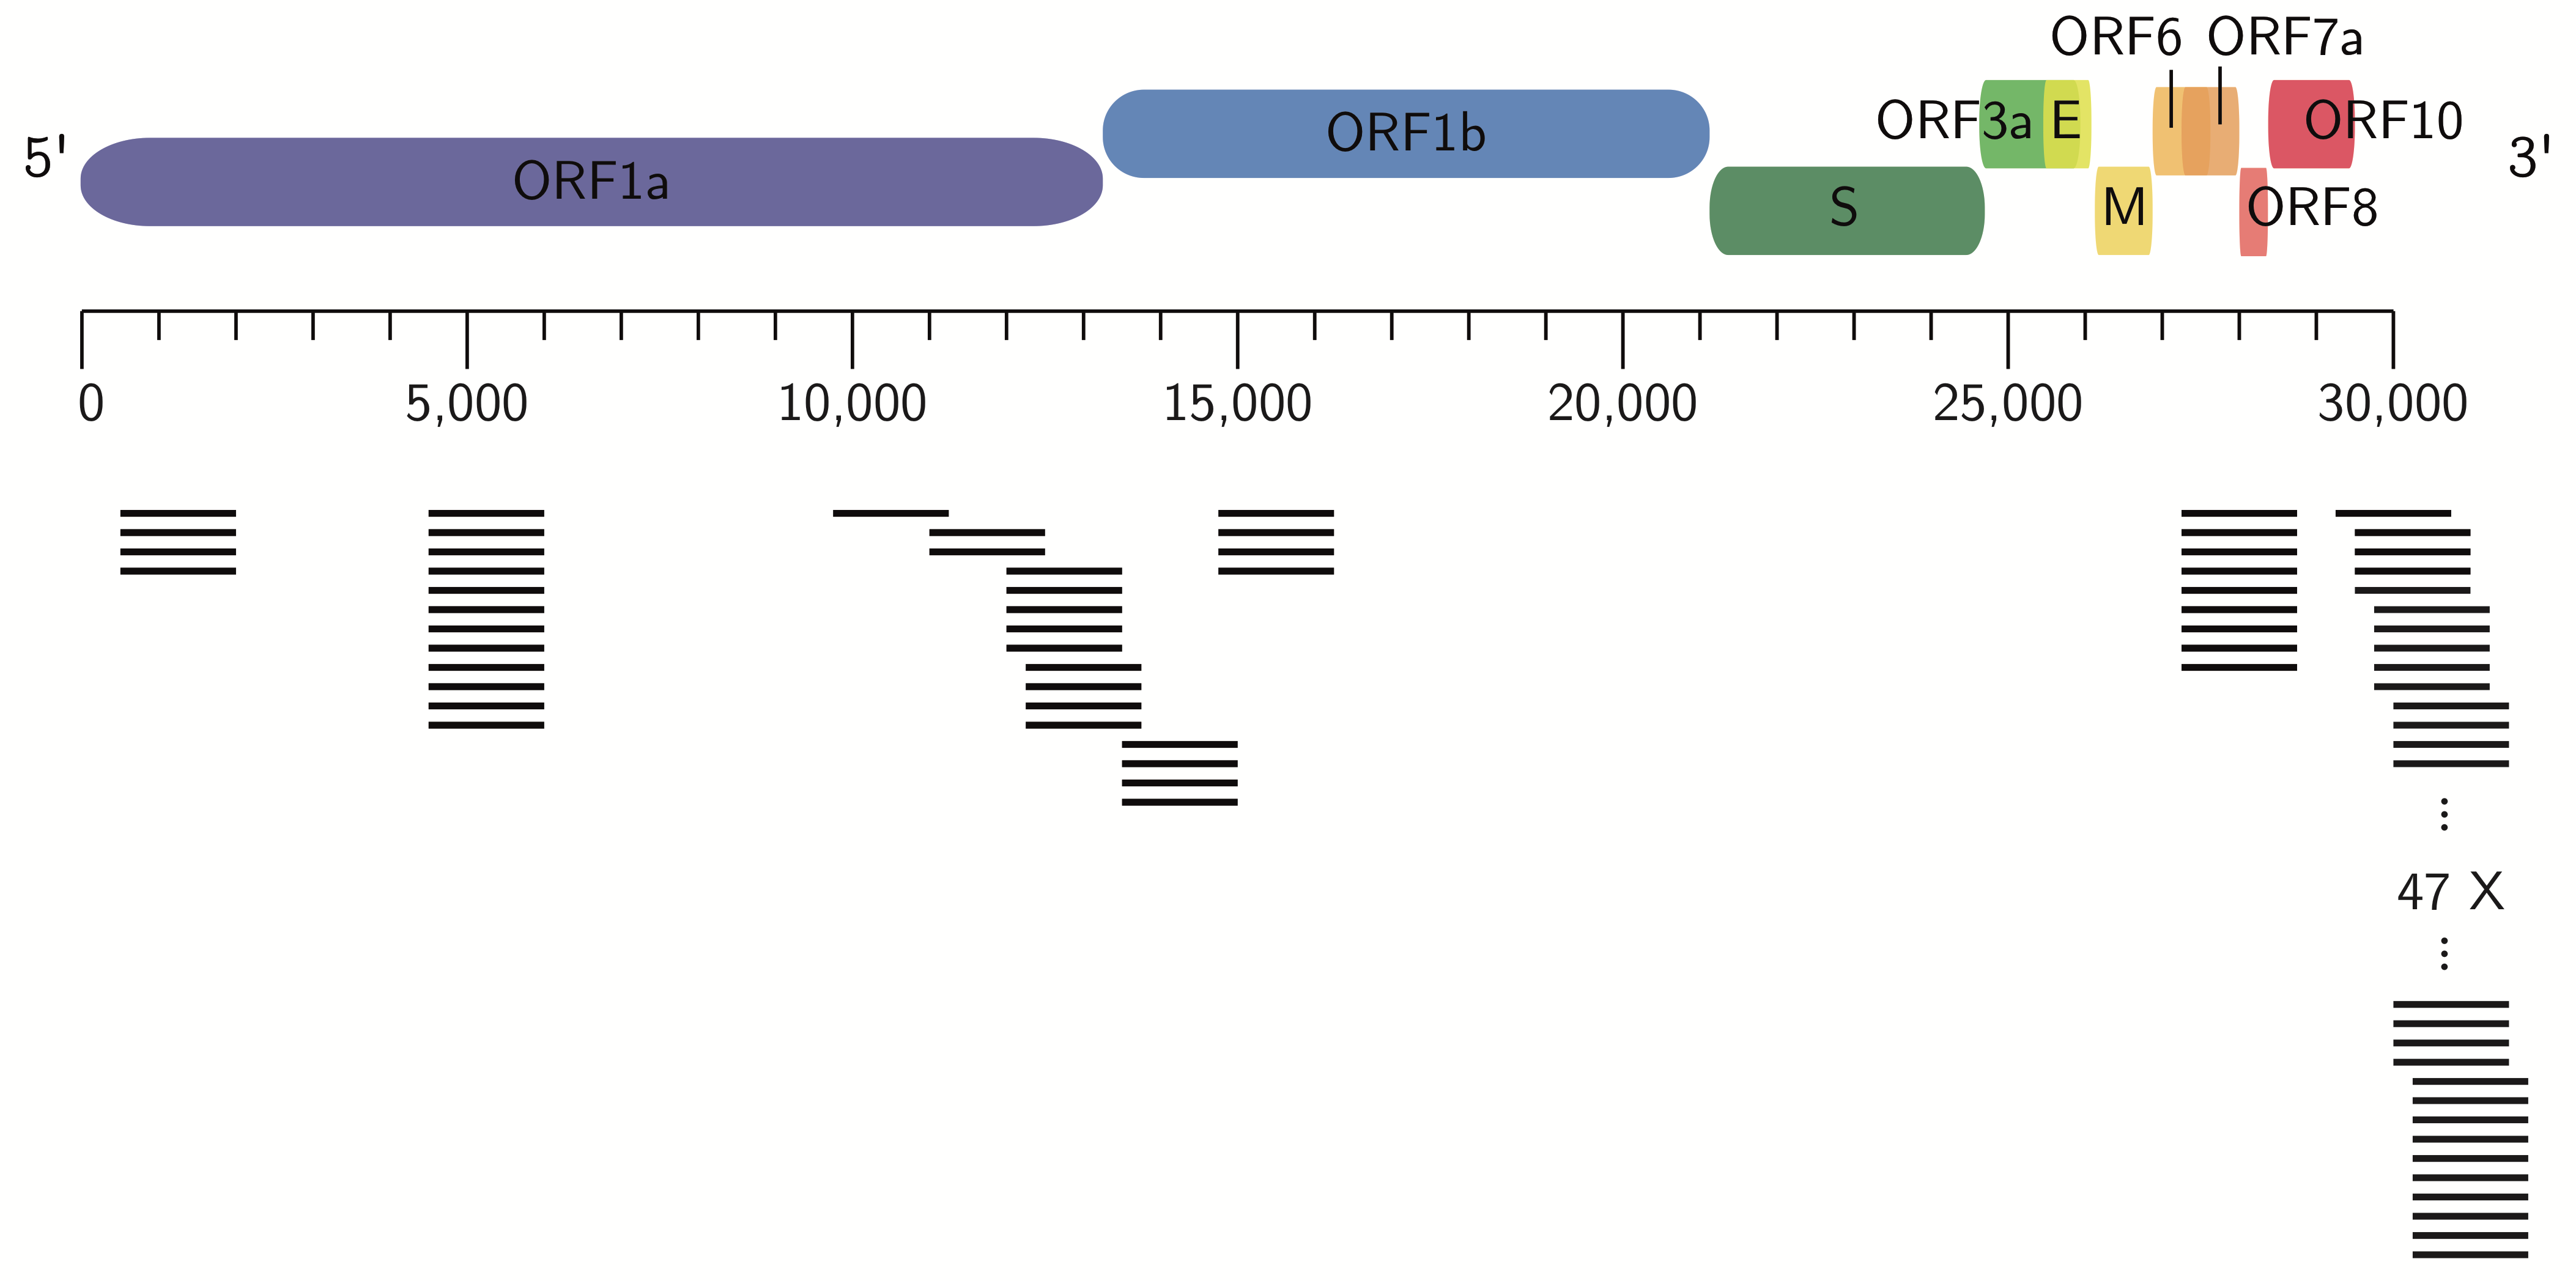
\includegraphics[scale=.4]{sarscov2_genome}
    \caption{Top: Genome of SARS-CoV-2 based on GenBank MN908947.3 and NCBI’s ORFfinder. Bottom: Transcript positions for proto-primers.} % Note that transcript lengths are scaled up relative to genome length for readability. 
\end{figure}
\end{frame}

% Demonstration on over-exploited ribosomal region: found unreported primer pairs \cite{PriSeT2021}

% \begin{frame}{Motivation: Lake Monitoring Project}
% \framesubtitle{Desiderium for Ongoing Protocol Enhancement II}
% \begin{enumerate}[II]
%     \item Structured digitalization of protocols, past studies
%     \begin{itemize}
%         \item Allow for meta-analyses 
%         % Example: Where is the data set used in study X?
%         % most effective primer for species X in terms of OTU size?
%         \item Shorten ramp-up period of new hires % researchers, interns, students, visiting researchers
%         \item Improve reproducability of analyses
%     \end{itemize}
   
% \end{enumerate}
% \begin{figure}\centering
%     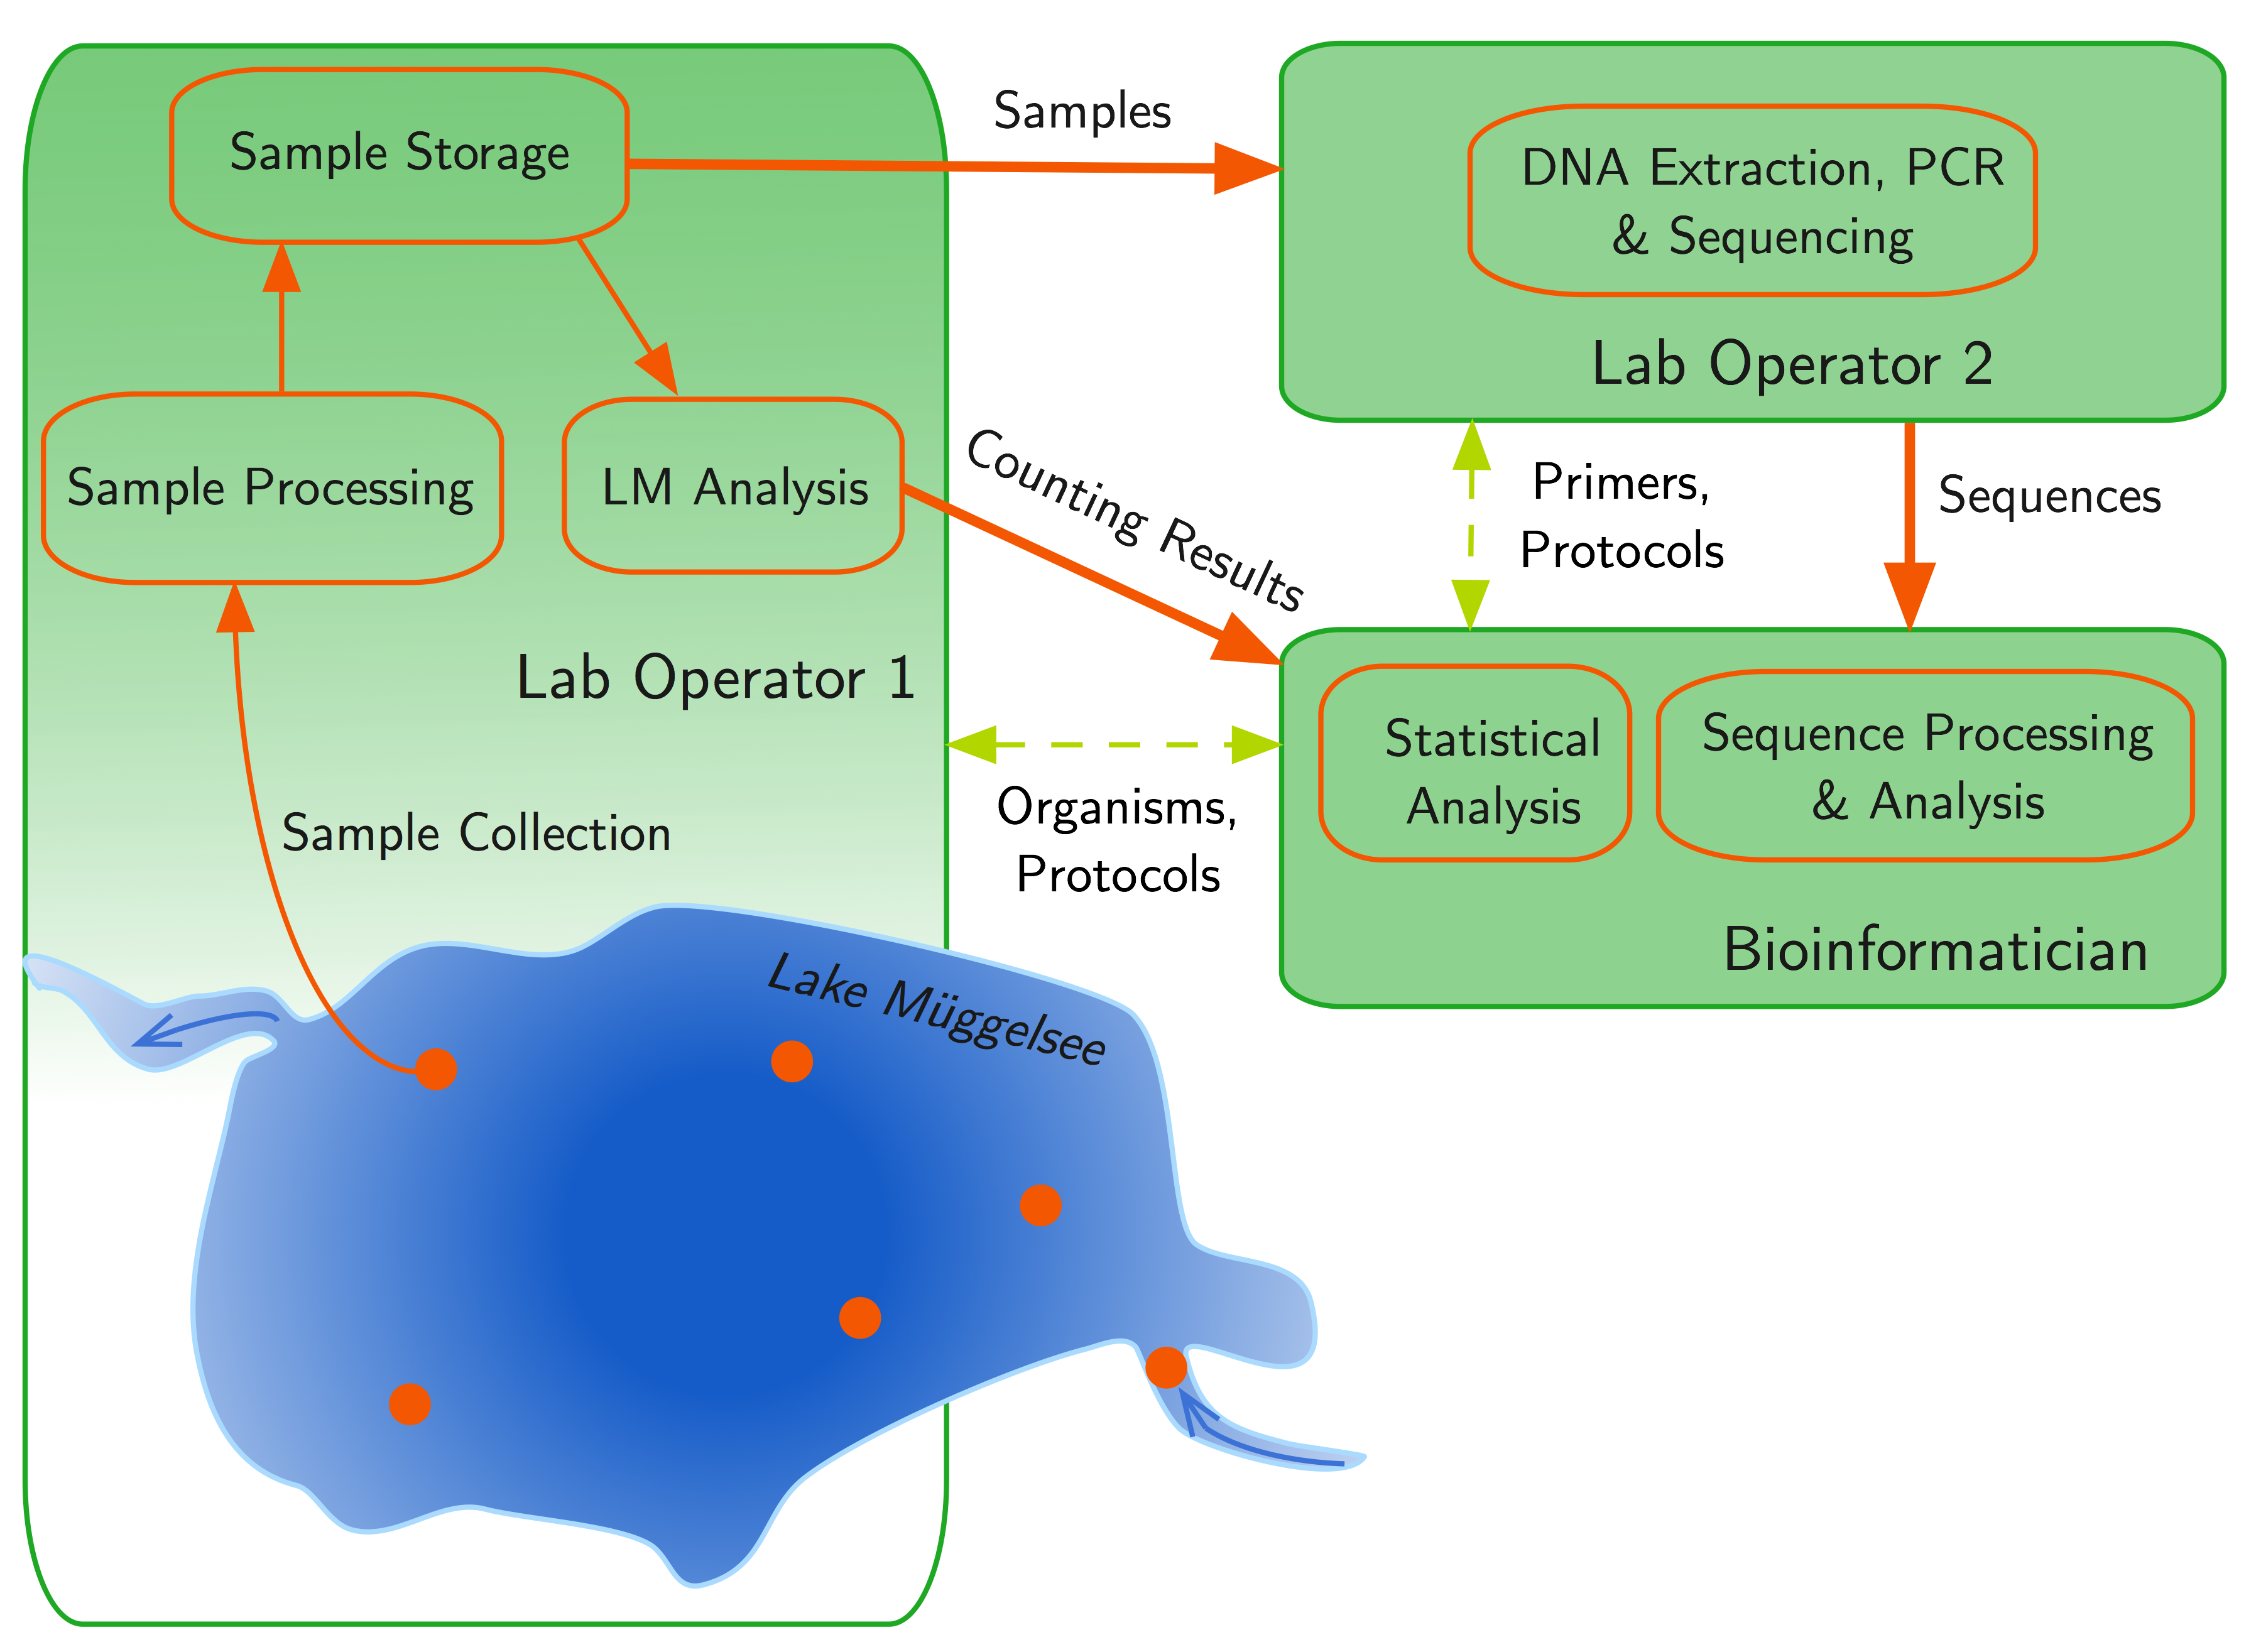
\includegraphics[scale=.45]{DB_flow}
%     \caption{Data transfer between lab operators and bioinformaticians.}
% \end{figure}
% Concretely:
%     * Problem: short stay of researchers, disjoint, splattered results, and the often quoted repeatability of experiments, each researcher has its own tool set, goes through the same evolution, sometimes rebuild pipelines to see if their results match -> slows down the pace
% * new types of analyses could be conducted if experimental setups, results are consolidated into a single scheme
% *  significant example here!
% * see DB schema
% * repeatability: serialisation of analysis pipelines
  
% \end{frame}


% \begin{frame}{II Database Schema}\framesubtitle{Data Consolidation and Querying}
%   \begin{figure}\centering
%     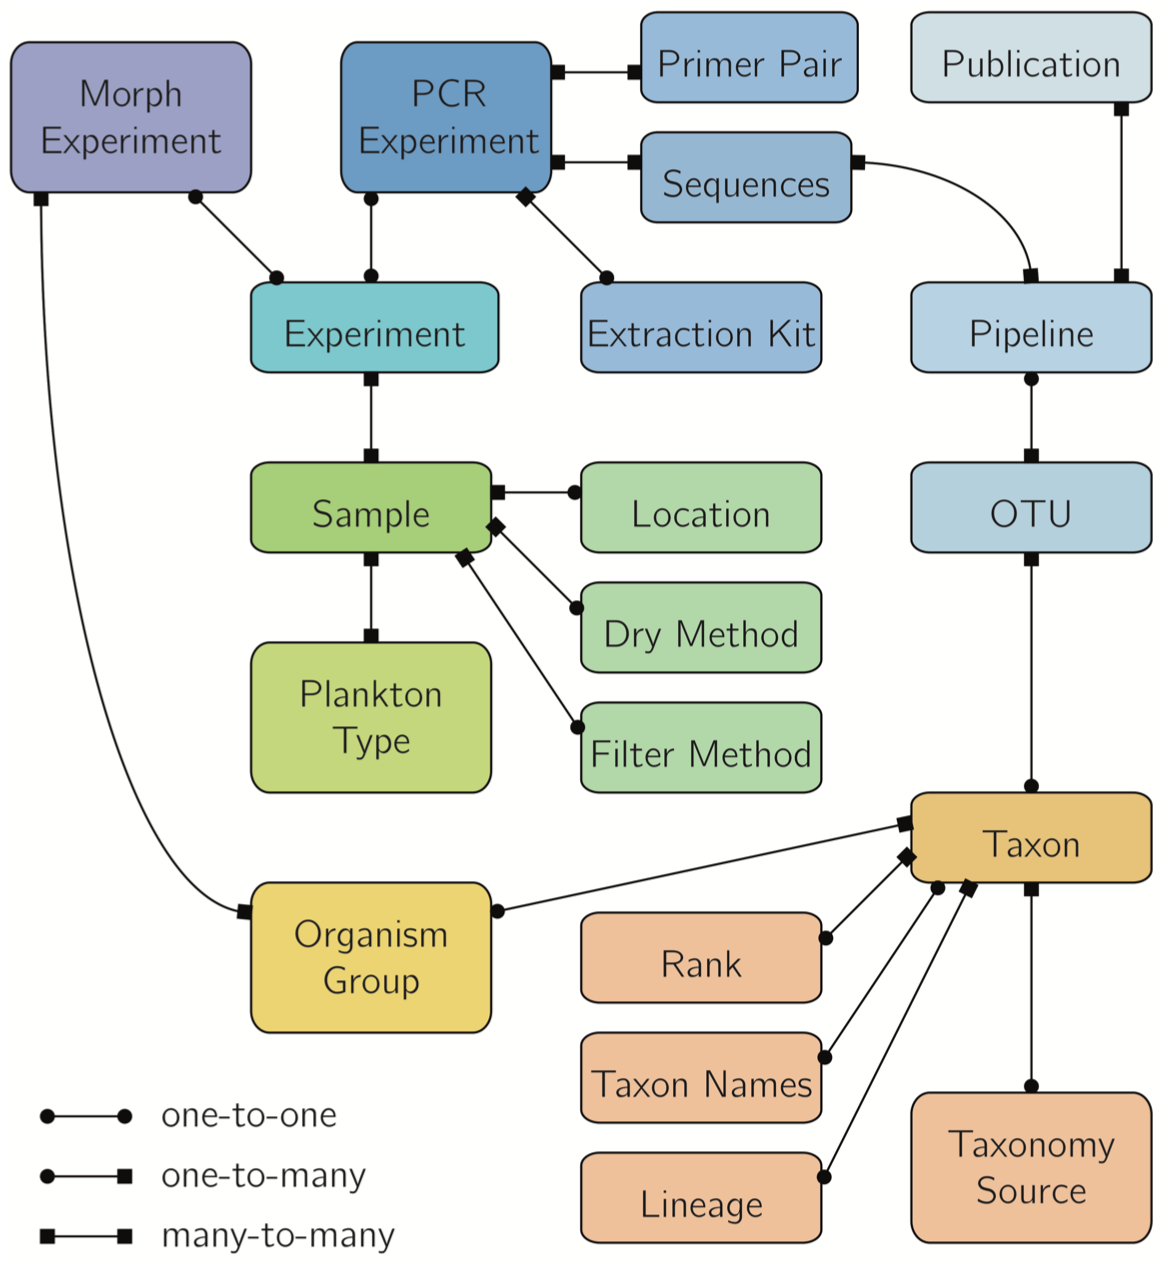
\includegraphics[scale=.3]{DB_schema}
%     \caption{Database schema \cite{PlanktonDB}}
%     \end{figure}
% \end{frame}


%----------- REFERENCES  -------------
%----------- No editing in references section ----------
%----------- edit only in References.bib ----------
	\begin{frame}[allowframebreaks]
		\justifying
		\frametitle{List of References}
		\printbibliography
	\end{frame}
%--------- THANK YOU Text --------------------------
	\begin{frame}
		\centering
		\begin{block}
			\scshape
				\begin{center}
					\large\emph{Thanks to} % I want to express my gratitude
				\end{center}
				\begin{itemize}
				    \item \underline{Commission}: Knut Reinert, Michael T. Monaghan, Katharina Jahn, Sandro Andreotti
				    \item \underline{Bioinformatics Group}: SeqAn Team
				    \item \underline{BeGenDiv}: Tatiana Semenova-Nelson, Camilla Mazzoni, Felix Heeger
				    \item \underline{IGB}: Rita Adrian, Justyna Wollinska, Ursula Newen
				    \item any many more
				\end{itemize}
		\end{block}
    \nocite{Burki2020, PriSeT2021}
	\end{frame}
%----------------------------------------------------

\section{Appendix}
\backupbegin

\begin{frame}{Appendix Motivation: Lake Monitoring Project}
\framesubtitle{Study Results: Unidentified Taxa for DNA ID}
$$
|\text{species} \in \{\text{Morph ID} \} \backslash \{ \text{DNA ID}\}|= 141
$$ 
%Morph ID species without DNA ID
\begin{table}[htpb]\centering\small
    \begin{tabular}{lcccccc}\toprule
        \multirow{3}{*}{Marker ID}&&\multicolumn{2}{c}{Species} && \multicolumn{2}{c}{{\it in silico} PCR}\\
        && Morphologically & Reference &&\multirow{2}{*}{Success} & \multirow{2}{*}{Failure}\\
        && identified & available/missing && &\\\toprule
        EUK15 && 144 & 70/74 && 68 (97 \%) & 2 (3 \%) \\
        EUK14 && 144 & 70/74 && 67 (96 \%) & 3 (4 \%)\\
        DIV4  && 144 & 70/74 && 48 (68 \%) & 22 (32 \%)\\\bottomrule
    \end{tabular}
    \caption{Results of {\it in silico} PCR for each primer set tested.}
    % Of the 144 taxa identified morphologically to species-level (without hybrids), 70 had database entries in either SILVA or NCBI's \emph{nt} dataset. {\it In silico} PCR success and failure rates were therefore calculated as \% of the 70 species that could have been recovered. Primer DIV4 exhibits a lower success rate on the complete species set (68 \%), but performs well on important phytoplankton groups
    \label{Tab:Tab_4}
\end{table}
\end{frame}

\begin{frame}{Appendix Evaluation on SARS-CoV-2}
\framesubtitle{qPCR Settings}

\begin{table}[htpb]\centering
\scriptsize
\begin{tabular}{lc}\toprule
Parameter&Settings SARS-CoV-2\\\midrule
$k$ & $[18:24]$ \\
$\tau$  [nt] & $[60:150]$\\
Tm  [\textdegree C] & $[55:63]$\\
GC [\%]& $[50:60]$\\
4-Runs of \cytosine{} or \guanine & yes\\
Self-Annealing & on\\\midrule
$\Delta $Tm  [K]& $5$\\
Cross-Annealing & on\\\bottomrule
\end{tabular}
\caption{Settings for qPCR.}\label{Tab:cfg3}
\end{table}
\end{frame}

\backupend

\end{document}
